\section{Architettura CUDA}

CUDA è l'architettura di elaborazione in parallelo progettata e sviluppata da
NVIDIA che sfrutta la potenza di calcolo delle GPU (Graphics Processing Units)
per aumentare le prestazioni nell'ambito del software computing.
L'elaborazione sta lentamente migrando verso il paradigma di
\textit{co-processing} su CPU e GPU il quale prevede che l'esecuzione della
gran parte del carico computazionale venga demandata alla GPU, e i risultati
presi nuovamente in carico dalla CPU.
\\
Questo nuovo tipo di architettura ha trovato immediato seguito nel settore
della ricerca scientifica, dato che ha contribuito in particolare alla nascita
e al miglioramento di software per la simulazione di fenomi fisici e
biologici.

\paragraph{Specifiche Hardware}

Generalmente l'hardware può cambiare con l'avvento di
nuove generazioni di GPU ma la struttura generale si basa sempre sul concetto di
Streaming Multiprocessors (SMs) \cite[p.~62]{nickolls2010gpu}

\begin{figure}[H]
    \centering
    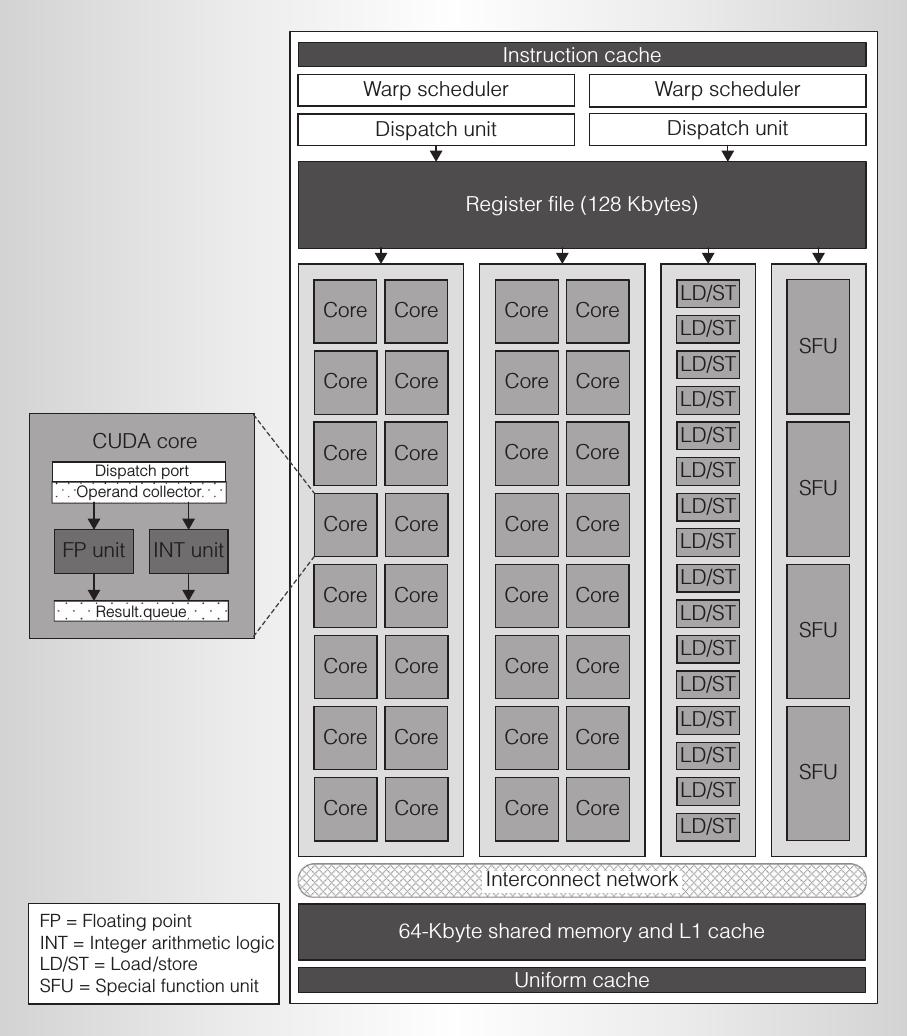
\includegraphics[scale=0.4]{fermi_sm}
    \caption{Streaming Multiprocessor dell'architettura Fermi 
        \cite[p.~63]{nickolls2010gpu}}
\end{figure}

\paragraph{Astrazione Software}

Dato che la struttura fisica delle schede è in continuo mutamento, NVIDIA ha
sviluppato delle API per dialogare con la GPU che sono indipendenti
dall'architettura del device utilizzato, rendendo così possibile lo sviluppo
di software portabile su molte schede che supportano CUDA.
\\
Il modello astratto definisce tre tipologie di oggetti:

\begin{itemize}
    \item
        \textbf{Thread}: singole unità di calcolo, eseguono il codice sorgente;
    \item
        \textbf{Thread block}: insieme logico di thread. I thread appartenenti
        allo stesso blocco hanno accesso ad un'area di memoria condivisa e
        accessibile solamente da loro (oltre alla memoria globale della GPU);
        inoltre è possibile ottenere un livello di sincronizzazione fra i thread
        del blocco;
    \item
        \textbf{Grid}: insieme logico di \textit{Thread block}. Non è stata
        prevista un'area di memoria condivisa da tutta la griglia e fino ad ora non
        esiste una primitiva per sincronizzare i blocchi di una specifica
        griglia, è quindi necessario procedere alla sincronizzazione di
        tutta la GPU.
\end{itemize}

\begin{figure}[H]
    \centering
    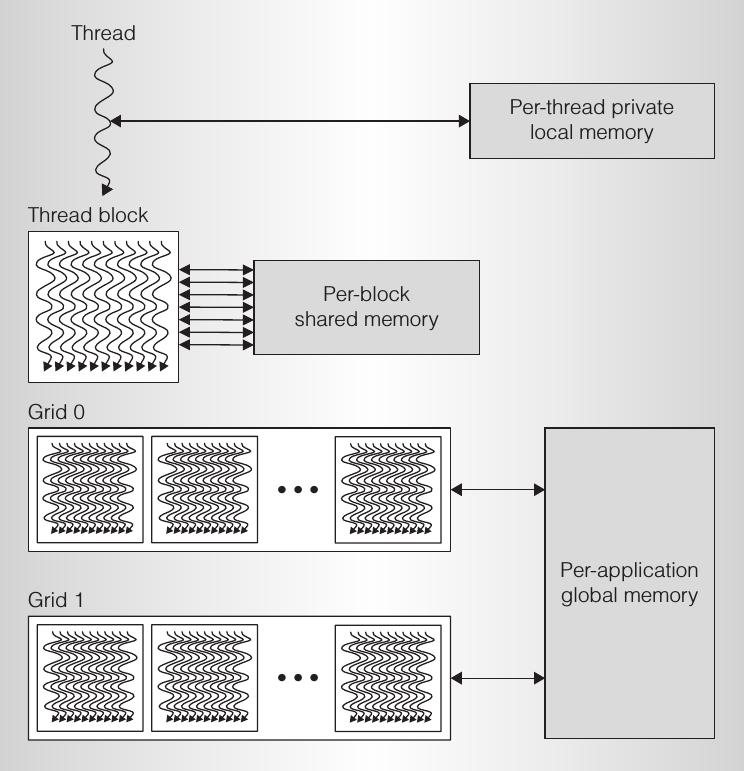
\includegraphics[scale=0.5]{cuda_astraction}
    \caption{Schema della gerarchia di \textit{Thread}, \textit{Thread block}, e
        \textit{Grid} \cite[p.~59]{nickolls2010gpu}}
\end{figure}

Le procedure che vengono eseguite sulla GPU vengono chiamate \textit{Kernel}
(identificabili grazie al prefisso \textit{\_\_global\_\_})
ed è possibile specificarne la dimensionalità, ovvero decidere quanti
\textit{Thread}, \textit{Thread block} e \textit{Grid} verranno assegnati
all'esecuzione del codice invocato.
\\
\lstinputlisting[label=kernel, language=C++, caption={Invocazione GPU kernel},
    style=custom]
    {Code/simple_kernel.cu}

Come è possibile notare nell'esempio di codice \ref{kernel}, stiamo invocando
l'esecuzione di un kernel specificando l'utilizzo di 8 \textit{Thread blocks} e
32 \textit{Thread} per blocco (se non viene specificato il numero delle
\textit{Grid} il valore di default è 1).
\\
Dunque in totale verranno utilizzati: $$1 * 8 * 32 = 256$$ thread per
l'esecuzione del kernel specificato.
\\
Questa suddivisione tra thread ci ritorna molto utile nell'elaborazione di
strutture dati come gli array, in quanto facilmente parallelizzabili.
Infatti è sufficiente invocare un kernel con numero di thread uguale
(o maggiore) al numero di elementi dell'array per ottenere il massimo grado
di parallelismo
\\
\lstinputlisting[label=threadid, language=C++,
    caption={Calcolo thread global id},
    style=custom]
    {Code/thread_id.cu}
